\subsection{Kalibrierung des B-Felds}
Die Messwerte zur Hysteresekurve der Kalibrierung des Magnetfelds sind in Tabelle \ref{tab:hysterese} notiert.
Die Werte werden in Abbildung \ref{fig:hysterese} dargestellt.
Da im folgenden Versuch kein höheres B-Feld als mit einem Strom von $I=\SI{15.5}{A}$ verwendet wird, lässt sich der verwendete Bereich linear fitten.
%
%
\begin{table}[h!]
  \centering
  \caption{Messdaten zur Kalibrierung des Magnetfelds}
  \label{tab:hysterese}
  \begin{tabular}{c c c c c c c c c c c}
    \toprule
%    \multicolumn{3}{c}{$f_{\text{1, theo}}=\SI{0.1}{m}$} & \multicolumn{3}{c}{$f_{\text{2, theo}}=\SI{0.05}{m}$}\\
      $I/$A   &   $B$/mT  &  $I$/A   & $B$/mT &  $I$/A   & $B$/mT &  $I$/A   & $B$/mT\\
      \midrule
      0     &   3.72    &   11    &   697.5   &    18    &   1012      &    7     &   436.7    \\
      1     &   76.65   &   12    &   763.7   &    17    &   981       &    6     &   386.6    \\
      2     &   132.1   &   13    &   820.0   &    16    &   943       &    5     &   313.5    \\
      3     &   198.2   &   14    &   872.5   &    15    &   926.2     &    4     &   250.0    \\
      4     &   261.7   &   15    &   922.3   &    14    &   873.9     &    3     &   178.7    \\
      5     &   321.9   &   16    &   964.1   &    13    &   811.2     &    2     &   118.7    \\
      6     &   390.6   &   17    &   974     &    12    &   756.8     &    1     &   53.88    \\
      7     &   453.4   &   18    &   1009    &    11    &   693.8     &    0     &   5.871    \\
      8     &   516.9   &   19    &   1039    &    10    &   612.8     &    -     &      -     \\
      9     &   578.5   &   20    &   1066    &    9     &   577.3     &    -     &      -     \\
      10    &   639.6   &   19    &   1038    &    8     &   503.5     &    -     &      -     \\
    \bottomrule
  \end{tabular}
\end{table}
%
%
\begin{figure}[h!]
  \centering
  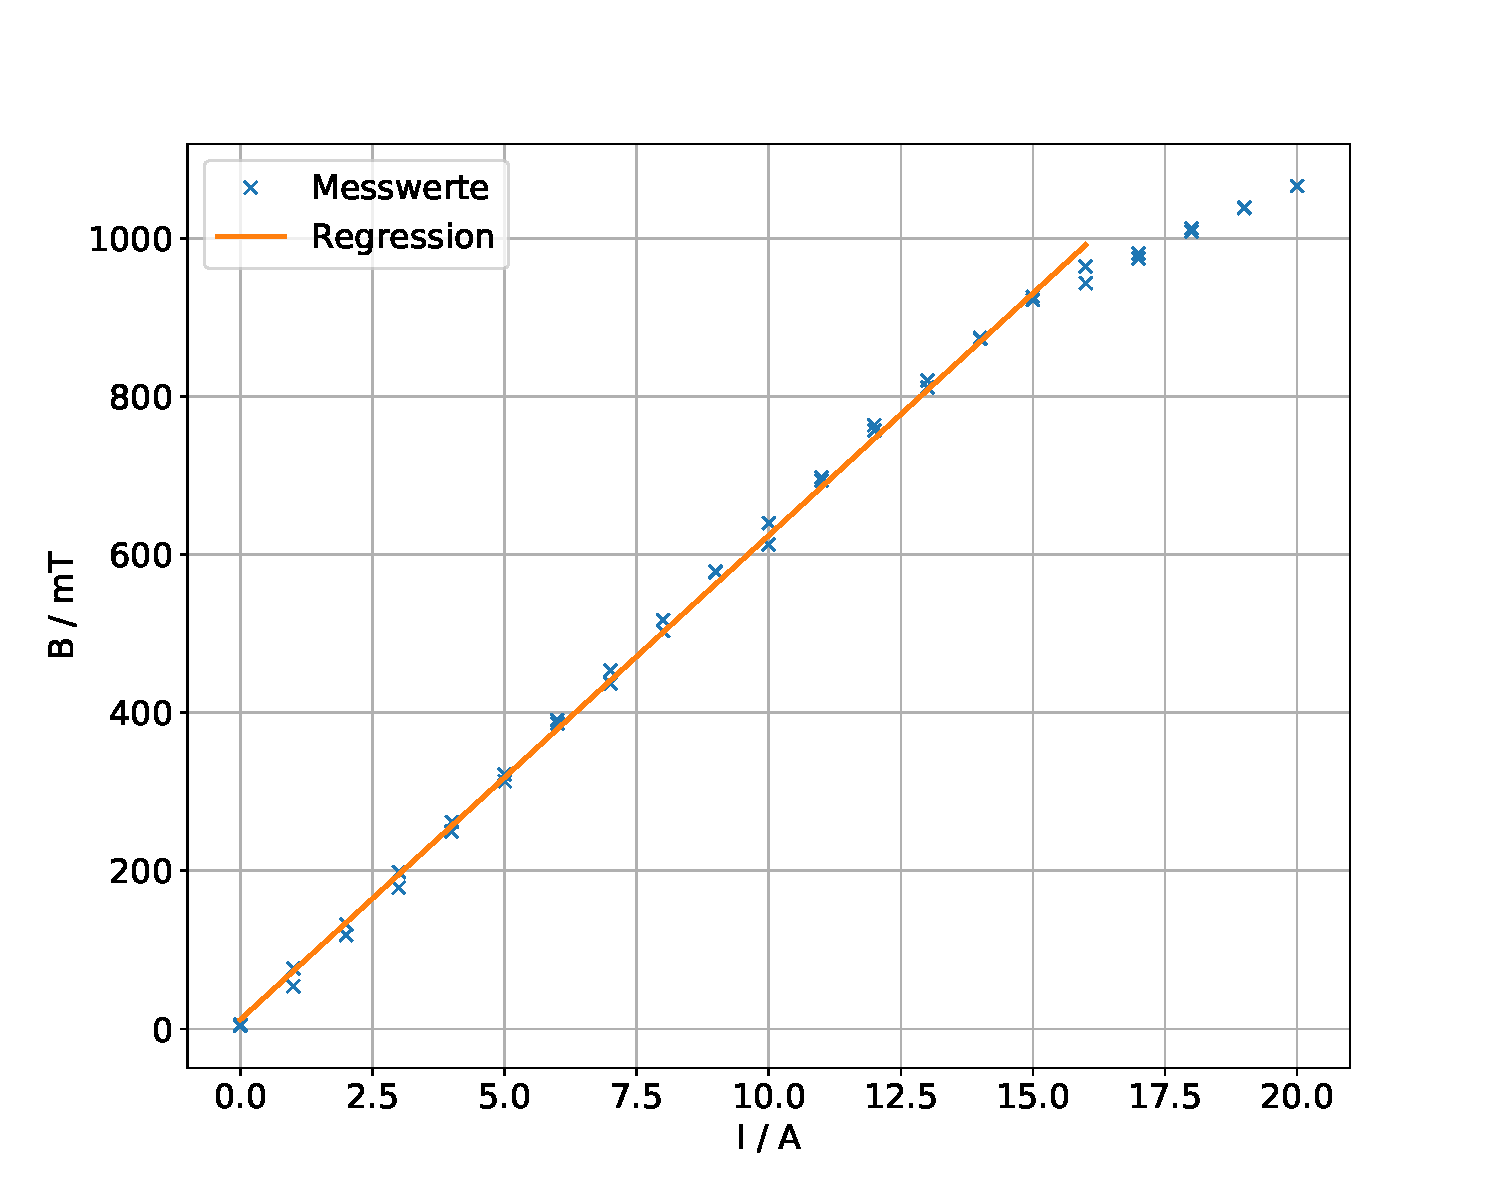
\includegraphics[width=\textwidth]{hysterese.pdf}
  \caption{Hysteresekurve der Kalibrierung des B-Felds}
  \label{fig:hysterese}
\end{figure}
Aus dem Fit der Form $B=aI+b$ mit Python 3.6.3 ($curve\_fit$) ergeben sich die Parameter $a$ und $b$:
\begin{align*}
   a &=& \SI{61.2 \pm 0.5}{\frac{mT}{A}} \\
   b &=& \SI{11.7 \pm 4.7}{mT}. \\
%   a &=& \SI{61.23769853 \pm 0.50050078}{\frac{mT}{A}} \\
%   b &=& \SI{11.74020588 \pm 4.6951124}{mT}. \\
\end{align*}

\FloatBarrier
\subsection{Rot: Normaler Zeeman-Effekt}
Die Werte zur Berechnung des Dispersionsgebietes der Lummer-Gehrke-Platte sind gegeben als
\begin{align*}
d         = \SI{4 e-03}{m}    \\
L         = \SI{120 e-03}{m}    \\
n(\SI{644}{nm})  = 1.4567    \\
n(\SI{480}{nm})  = 1.4635    \\
\end{align*}
Damit ergibt sich für das rote Licht ($\SI{644}{nm}$) das Dispersionsgebiet
\begin{equation*}
  \Delta \lambda_D = \SI{4.89e-11}{m}.
%  \Delta \lambda_D = \SI{4.8912559475e-11}{m}.
\end{equation*}
Die Abstände zwischen den Linien werden nach entsprechender Bearbeitung des Kontrasts und der Belichtung ausgewertet.
Die Messwerte sind in Tabelle \ref{tab:rot} notiert.
Es wird das Verhältnis der Aufspaltung bei angelegtem B-Feld zum Abstand der Linien ohne angelegtes B-Feld $\frac{\delta s_{1}}{\Delta s}$ berechnet.
Mit dem Verhältnis und dem Dispersionsgebiet ergibt sich die Wellenlängenverschiebung $\delta \lambda$.
%
%
\begin{table}[h!]
  \centering
  \caption{Messdaten zum normalen Zeeman-Effekt}
  \label{tab:rot}
  \begin{tabular}{c c c c c c c c c c c}
    \toprule
%    \multicolumn{3}{c}{$f_{\text{1, theo}}=\SI{0.1}{m}$} & \multicolumn{3}{c}{$f_{\text{2, theo}}=\SI{0.05}{m}$}\\

      $\Delta s$/Pixel & $\delta s_{1}$/Pixel & $\frac{\delta s_{1}}{\Delta s}$ & $ \delta \lambda_{1} $  \\
      \midrule
      158       &   70            & 0.443           &     1.084 e-11    \\
      160       &   76            & 0.475           &     1.162 e-11    \\
      169       &   79            & 0.468           &     1.143 e-11    \\
      173       &   81            & 0.468           &     1.145 e-11    \\
      187       &   82            & 0.439           &     1.072 e-11    \\
      192       &   89            & 0.464           &     1.134 e-11    \\
      192       &   88            & 0.458           &     1.121 e-11    \\
      200       &   93            & 0.465           &     1.137 e-11    \\
      212       &   96            & 0.453           &     1.108 e-11    \\
      224       &   102           & 0.455           &     1.114 e-11    \\
      238       &   106           & 0.445           &     1.089 e-11    \\
      256       &   116           & 0.453           &     1.108 e-11    \\
    \bottomrule
  \end{tabular}
\end{table}
%
%
Als gemittelte Wellenlängenverschiebung ergibt sich
\begin{equation*}
  \overline{\delta \lambda} = \SI{1.12 \pm 0.03 e-11}{m}.
%  \overline{\delta \lambda} = \SI{1.11801268255 \pm 0.0261742187244 e-11}{m}.
\end{equation*}
Das verwendetete Magnetfeld beim Strom $I=\SI{9.5}{A}$ hat die Stärke
\begin{equation*}
  B= \SI{593.5 \pm 6.7}{mT} = \SI{0.5935 \pm 0.0067}{T}.
%  B= \SI{593.498341915 \pm 6.68220012246}{mT} = \SI{0.593498341915 \pm 0.00668220012246}{T}.
\end{equation*}
Der Fehler wird als Gaußfehler berechnet.
Die Energie wird über die Energieänderung und \eqref{eqn:normal} wie folgt berechnet:
\begin{equation}
  \notag
  \Delta E = | E \left( \lambda_{0} + \overline{\delta \lambda} \right) - E \left( \lambda_{0} \right) |
           = \left| E( \lambda_{0}) + \frac{\partial E}{\partial \lambda}\overline{\delta \lambda} - E \left( \lambda_{0} \right) \right|
           = \left| \frac{\partial E}{\partial \lambda}\overline{\delta \lambda} \right|
           = \frac{h c}{ \lambda^2 } \overline{\delta \lambda }
           \label{eqn:energie}
\end{equation}
Mit Gleichung \eqref{eqn:normal} und der Gaußschen Fehlerfortpflanzung ergibt sich
\begin{align*}
  m &= \frac{h c}{\mu_B B \lambda^2 } \overline{\delta \lambda } \\
    &= \SI{-0.724 \pm 0.012}{}.
%    &= \SI{-0.7237389360859435 \pm 0.0121114490656}{}.
\end{align*}
%Exp nach Josh: 1.08
%Theo nach Josh: 1

\FloatBarrier
\subsection{Blau: Anormaler Zeeman-Effekt}
Als Dispersionsgebiet ergibt sich für das blaue Licht ($\SI{480}{nm}$):
\begin{equation*}
  \Delta \lambda_D = \SI{2.70e-11}{m}.
%  \Delta \lambda_D = \SI{2.69520209289e-11}{m}.
\end{equation*}
Die aus den Bildern aufgenommenen Messwerte sind in Tabelle \ref{tab:blau} notiert.
Zunächst wird nun das Verhältnis aus den Messwerten der Aufspaltungen mit entsprechender Polarisation ($2 \widehat{=} \text{zirkular}$, $3 \widehat{=} \text{linear}$) zur unpolarisierten Messreihe ohne angelegtes B-Feld $\delta s_{2}/\Delta s$ bzw. $\delta s_{3}/ \Delta s$ ausgerechnet.
Mit dem Verhältnis und dem Dispersionsgebiet wird die Wellenlängenverschiebung $\delta \lambda$ für beide Polarisationen berechnet.
%
%
\begin{table}[h!]
  \centering
  \caption{Messdaten zum anormalen Zeeman-Effekt}
  \label{tab:blau}
  \begin{tabular}{c c c c c c c c c c c}
    \toprule
%    \multicolumn{3}{c}{$f_{\text{1, theo}}=\SI{0.1}{m}$} & \multicolumn{3}{c}{$f_{\text{2, theo}}=\SI{0.05}{m}$}\\

      $\Delta s$/Pixel & $\delta s_{2}$/Pixel & $\delta s_{3}$/Pixel & $\frac{\delta s_{2}}{\Delta s}$ & $\frac{\delta s_{3}}{\Delta s}$  & $ \delta \lambda_{2} $ &  $\delta \lambda_{3}$    \\
      \midrule
      140   &   49    &   50    &   0.350   &     0.357     &   4.717 e-12   & 4.813e-12  \\
      154   &   52    &   65    &   0.338   &     0.422     &   4.550 e-12   & 5.688e-12  \\
      173   &   54    &   63    &   0.312   &     0.364     &   4.206 e-12   & 4.908e-12  \\
      177   &   62    &   57    &   0.350   &     0.322     &   4.720 e-12   & 4.340e-12  \\
      187   &   64    &   63    &   0.342   &     0.337     &   4.612 e-12   & 4.540e-12  \\
      197   &   68    &   69    &   0.345   &     0.350     &   4.652 e-12   & 4.720e-12  \\
      209   &   72    &   66    &   0.345   &     0.316     &   4.643 e-12   & 4.256e-12  \\
      233   &   74    &   74    &   0.318   &     0.318     &   4.280 e-12   & 4.280e-12  \\
      250   &   82    &   80    &   0.328   &     0.320     &   4.420 e-12   & 4.312e-12  \\
      282   &   89    &   90    &   0.316   &     0.319     &   4.253 e-12   & 4.301e-12  \\
      321   &   103   &   97    &   0.321   &     0.302     &   4.324 e-12   & 4.072e-12  \\
      399   &   120   &   135   &   0.301   &     0.338     &   4.053 e-12   & 4.560e-12  \\
    \bottomrule
  \end{tabular}
\end{table}
%
%
Der Mittelwert der Wellenlängenverschiebung $\delta s$ und der zugehörige Fehler als Standardabweichung werden mit der numpy-Bibliothek in Python (numpy.mean, numpy.std) berechnet.
Es ergeben sich folgende Werte:
\begin{align*}
  \text{zirkular}  &&  \overline{\delta \lambda} &=& \SI{4.5 \pm 0.2 e-12}{m} \\
  \text{linear}    &&  \overline{\delta \lambda} &=& \SI{4.6 \pm 0.4 e-12}{m}. \\
%  \text{zirkular}  &&  \overline{\delta \lambda} &=& \SI{4.45250571816 \pm 0.215951778182 e-12}{m} \\
%  \text{linear}    &&  \overline{\delta \lambda} &=& \SI{4.56570632339 \pm 0.415188327987 e-12}{m}. \\
\end{align*}
Der magnetfelderzeugende Strom wird bei der Messung erhöht.
Es ergeben sich folgende Magnetfelder:
\begin{align*}
  \text{zirkular}  &&   I &=& \SI{5}{A}     && B &=& \SI{317.9 \pm 5.3}{mT}\\
  \text{linear}    &&   I &=& \SI{15.5}{A}  && B &=& \SI{960.9 \pm 9.1}{mT}.\\
%  \text{zirkular}  &&   I &=& \SI{5}{A}     && B &=& \SI{317.92869853 \pm 5.32039530657}{mT}\\
%  \text{linear}    &&   I &=& \SI{15.5}{A}  && B &=& \SI{960.924533095 \pm 9.06790786751}{mT}.\\
\end{align*}
Die Energie ergibt sich durch Gleichung \eqref{eqn:anormal} und $E= h \nu$.
$E_0$ ist die Energie des Lichts bei $B=0$ mit $E_0=h \nu = \frac{hc}{\lambda}= \SI{4.14e-19}{J}=\SI{2.58}{eV}$
%Dabei ist für den vorliegenden Übergang $g_{J_i}=\frac{3}{2}$ und $g_{J_j}=2$:
Analog zu \eqref{eqn:energie} lässt sich die Energieänderung und der Landé-Faktor des Übergangs berechnen.
Für die zirkulare Polarisation ergibt sich
\begin{equation*}
  g_{ij} = \SI{-1.30 \pm 0.02}{}.
%  g_{ij} = \SI{-1.301971289913896 \pm 0.0217879102207}{}.
\end{equation*}
%Exp nach Josh: 2.0
%Theo nach Josh: 2
Für die lineare Polarisation
\begin{equation*}
  g_{ij} = \SI{-0.442 \pm 0.004}{}.
%  g_{ij} = \SI{-0.44171825295855427 \pm 0.00416834026323}{}.
\end{equation*}
%Exp nach Josh: 0.55
%Theo nach Josh: 0.5

\FloatBarrier
%\end{landscape}
%\end{document}
